\documentclass[main]{subfiles}
\begin{document}

\section{提案手法}
\subsection{CMT\cite{xiao2023multi}}
\label{提案手法:CMT}
CMTはMTの教師予測に対し，クリップ及びフレーム単位で閾値を適用する．
まず，弱予測の結果に基づき，閾値未満の予測を同区間の強予測を含め学習対象から除外する．
次に，閾値を上回る予測に対しては，イベント種別に応じた窓幅のメディアンフィルタを適用し，平滑化と外れ値の除去を行う． 
損失計算においては，二値化された信頼度マスクを重みとして，教師・生徒モデル間の二値交差エントロピー（Binary Cross Entropy; BCE）誤差を最小化する．\par

本実験環境において，CMTはPSDS2を向上させた一方，PSDS1を低下させた．
これは，低確信度の予測を損失計算から一律に除外することで，「イベントが存在しない」という負例の情報が学習されず，結果として時間境界の推定精度が損なわれたためと考えられる．\par

そこで本研究では，負例を学習に組み込み，PSDS2の改善を維持しつつ，PSDS1の向上を図る．
具体的には，確率0.7以上を「信頼できる正例」，0.3以下を「信頼できる負例」とし，不確実な中間領域の予測のみを学習から除外する．
さらに，正負例のサンプル不均衡による精度低下を回避するため，サンプル数の比率に基づく損失の正規化を行う．

\subsection{MixStyle\cite{zhou2021domain}}
\label{提案手法:MixStyle}
\begin{figure}[H]
    \centering
    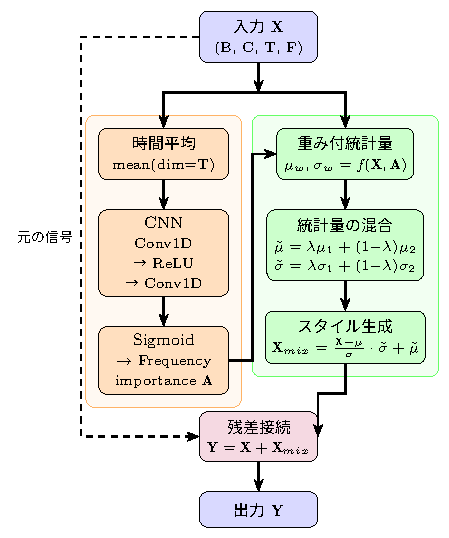
\includegraphics[width=0.6\columnwidth]{figures/mixstyle.pdf}
    \caption{オレンジの領域がCNN，緑がMixStyle，そして赤が残差接続で，それぞれ本文の1から3に対応する．}
    \label{fig:mixstyle}
\end{figure}

MixStyleは，画像認識におけるドメイン汎化のために提案されたデータ拡張手法である．
画像分野では空間情報に着目し，チャネルごとの平均と標準偏差をドメイン固有のスタイル統計量として抽出し，他データと混合する．
一方で，音響信号は時間と周波数の次元を持ち，ドメイン情報は主に周波数領域に局在することが示唆されている\cite{kim2022domain}．
この特性に基づき，Xiaoら\cite{xiao2024fmsg}は時間方向の統計量を計算し，周波数軸に沿って混合する手法を提案した．
これにより，元データに含まれる意味的な情報を保持しつつ，多様なドメインスタイルを生成し，特定ドメインへの過剰な適合を防ぐ．\par

しかし先行研究\cite{xiao2024fmsg}では，MixStyleと周波数方向の注意機構が結合されているものの，その統合プロセスや相互作用は詳らかにされていない．
本研究では，周波数領域におけるドメイン汎化をより軽量に実現するため，MixStyleとCNNを統合する．
本手法は以下の3段階で構成され，重要な信号情報を損なうことなく効果的なドメイン適応を実現する． 
\begin{enumerate}
\item CNNによる重要周波数帯域の特定 
\item 重要度を考慮した重み付き統計量の混合 
\item 残差接続による原信号のドメイン情報の保持 
\end{enumerate}

具体的なアーキテクチャを図\ref{fig:mixstyle}に示す．
MixStyleの適用は\cite{xiao2024fmsg}に倣い，CNNへの入力直前，及び第1・第2畳み込み層直後の特徴量を対象とした．%図\ref{fig:cnn}ではInput，ブロック1，2の後となる．
ハイパーパラメータは\cite{zhou2021domain}を参照し，適用確率を$p=0.5$，ベータ分布のパラメータを$\alpha=0.1$に設定した．
混合対象であるスタイル統計量は，ミニバッチ内からランダムに選択される．
本実験では，ドメイン汎化の対象として合成音（DESED）と実録音（MAESTRO Real）を扱うが，
MixStyleはランダムな選択であっても十分な正則化効果が得られることが報告されている\cite{zhou2021domain}．
したがって，計算コストと実装の簡便性を優先し，異なるスタイルを持つデータを選択するのではなく，バッチ内ランダム選択による混合を行った．\par

提案手法の詳細を以下に述べる．入力特徴量を $X \in \mathbb{R}^{B \times C \times T \times F}$ とする．
まず，時間方向の平均を算出することで時間情報を集約し，周波数特徴記述子 $Z \in \mathbb{R}^{B \times C \times F}$ を得る．
$$Z_{b,c,f} = \frac{1}{T} \sum_{t=1}^{T} X_{b,c,t,f}$$

次に，$Z$に対してCNNを適用し，周波数ごとの重要度マップ $A \in \mathbb{R}^{B \times C \times 1 \times F}$ を生成する．
ネットワーク構成には，カーネルサイズ3の1次元畳み込み層，ReLU関数$\delta$ ，及びカーネルサイズ1の1次元畳み込み層からなるボトルネック構造を採用した．
最終層にはSigmoid関数$\sigma$を適用し，出力を $(0, 1)$ の範囲に正規化する．
$$A = \sigma(W_2 \cdot \delta(W_1 \cdot Z))$$

ここで，$W_1, W_2$ は畳み込み層の重みを表す．
なお，学習初期の勾配消失を抑制し，統計量の混合を促進するため，最終層のバイアスは $1.0$ で初期化した．\par

推定された重要度 $A$ に基づき，周波数ごとの重み付き平均 $\mu$ 及び重み付き標準偏差 $\sigma$ を算出する．
これらを用いて正規化及び異種ドメイン（ミニバッチ内の他サンプル）との混合を行い，新たな特徴量 $X_{mix}$ を生成する．
最後に，元の信号情報の損失を防ぎつつドメイン不変性を獲得するため，下式に示す残差構造を導入する．
$$Y = X + \text{MixStyle}(X, A)$$
% この残差構造により，モデルは主要な音響イベント情報を保持したまま，MixStyleによるドメイン変動に対する頑健性を効率的に学習できる．\par
\end{document}